%=======================================================
%	PACKAGES AND THEMES
%=======================================================
\documentclass[8pt]{beamer}
\mode<presentation> {
\usepackage{etex}
\usetheme{Boadilla}
\definecolor{navyblue}{rgb}{0.0, 0.0, 0.5}
\definecolor{dkgreen}{rgb}{0,0.6,0}
\definecolor{gray}{RGB}{64, 64, 64}
\definecolor{mauve}{rgb}{0.58,0,0.82}
\usecolortheme[named = navyblue]{structure}
\setbeamercolor{normal text}{fg = gray}
\setbeamercolor{frametitle}{fg = white, bg = navyblue}
\setbeamerfont{framesubtitle}{size = \normalsize}
\setbeamerfont{caption}{size=\footnotesize}
\setbeamercolor{page number in head/foot}{fg = gray}
\setbeamertemplate{footline}%[frame number]
}


\usepackage{graphicx} % Allows including images
\usepackage{booktabs} % Allows the use of \toprule, \midrule and \bottomrule in tables
\usepackage{multicol}
\usepackage[export]{adjustbox}
\usepackage{colortbl}
\usepackage{graphicx} 

\usepackage{tikz}
\usepackage{fancybox}
\usepackage[absolute, overlay]{textpos}
\usepackage{multirow}
\usepackage{siunitx}
\usepackage{tcolorbox}


\usepackage{tikz}
\usepackage{calc}
\newlength{\outerradius}
\newlength{\innerradius}
\setlength{\outerradius}{0.50cm}
\setlength{\innerradius}{0.35cm}

%Damit wir Quellcode nutzen können.
\usepackage{listings}
\lstset{numbers=left,
	numberstyle=\tiny,
	numbersep=5pt,
	breaklines=true,
	showstringspaces=false,
	frame=l ,
	xleftmargin=15pt,
	xrightmargin=15pt,
	basicstyle=\ttfamily\scriptsize,
	stepnumber=1,
	keywordstyle=\color{blue},          % keyword style
  	commentstyle=\color{dkgreen},       % comment style
  	stringstyle=\color{mauve}         % string literal style
}
%Sprache Festelegen
\lstset{language=R}


%=======================================================
%	TITLE PAGE
%=======================================================

\title{\textbf{Descriptive Network Analysis C}}

\author{Dr David Eggleton}

\institute
{
SPRU (Science Policy Research Unit) \\
Business School\\
University of Sussex \\

\medskip

\medskip

\medskip

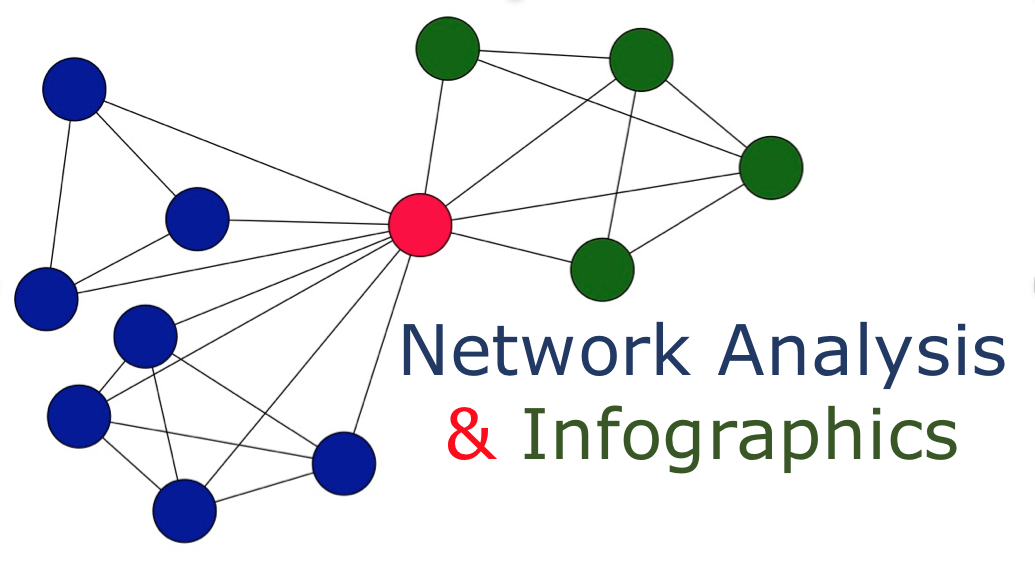
\includegraphics[width=2.5cm]{../_shared_pics/logo}

\medskip

\textit{{\color{dkgreen}{Week 6}}}\\
}


\date{} % Date, can be changed to a custom date

\begin{document}

\begin{frame}
\titlepage % Print the title page as the first slide

\begin{textblock*}{10pt}(0pt, 0.9\textheight)

\includegraphics[width=4cm]{../_shared_pics/SPRU.png}
\end{textblock*}

\end{frame}


%=======================================================
%	Learning outcomes
%=======================================================

\begin{frame}
\frametitle{Learning Outcomes}

\centering
\footnotesize
\begin{tabular}{lp{5.5cm}l}
\toprule
\multicolumn{2}{l}{\textbf{Learning outcome}} & \textbf{Assessment mode}\\
\hline
\\
1 & 
Explain the concept of network and list the main network indicators & 
ESS\\
\\
2 & 
Describe and apply the major techniques for the collection of network data and their statistical analysis & 
ESS, GPN + GWS\\
\\
\rowcolor{green!20}3 & 
Identify the main characteristics of networks by means of network measures  & 
ESS, GPN + GWS\\
\\
4 &
Employ network analysis techniques to produce network data-based infographics & 
GPN + GWS\\
\\
\bottomrule
\multicolumn{3}{l}{Note: ESS: Essay; GPN: Group Presentation; GWS: Group Written Submission}\\
\end{tabular}

\end{frame}

%------------------------------------------------


%=======================================================
%	Node-level measures
%=======================================================
\section{Node-level measures}
%------------------------------------------------

\bgroup
\setbeamercolor{background canvas}{bg = navyblue}
\begin{frame}[plain]{}
\begin{center}
\color{white}{\Huge\insertsection}
\end{center}
\end{frame}
\egroup

%------------------------------------------------

\begin{frame}
\frametitle{\insertsection}
\framesubtitle{Overview}

\begin{columns}

\column{.45\textwidth} 
\begin{enumerate}
\item Centrality
    \begin{itemize}
    \item Degree
    \item Closeness
    \item Betweenness
    \item Centralisation
    \item Bonacich's centrality
    \item Weighted centrality
    \end{itemize}
    
\medskip    

\item Brokerage
    \begin{itemize} 
    \item Brokerage roles
    \item Effective network size/efficiency
    \item Constraint
    \end{itemize}
\end{enumerate}


\column{.45\textwidth} 
\centering
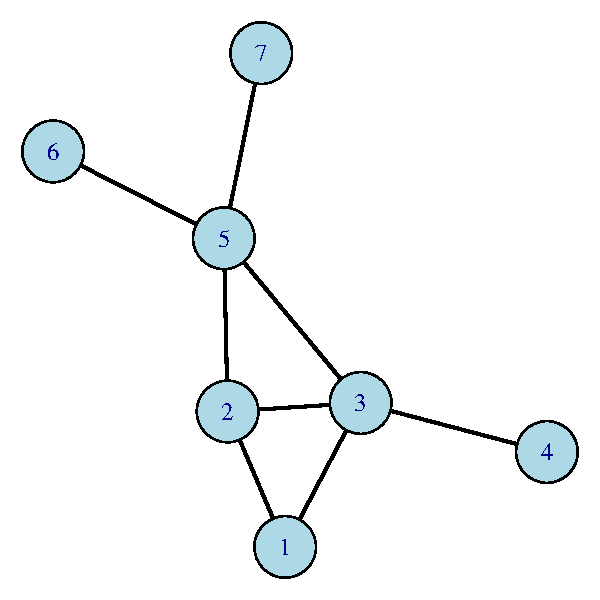
\includegraphics[width=5cm]{base}\\
\color{red}{\footnotesize Note: We will focus on\\ undirected and unweighted networks}

            
\end{columns}

\end{frame}

%------------------------------------------------
\subsection{Brokerage}
%------------------------------------------------

\begin{frame}
\frametitle{\insertsection}
\framesubtitle{\insertsubsection}

\begin{columns}

\column{.45\textwidth} 
\begin{itemize}
\item The concept of brokerage is related to the {\color{blue}{absence of ties}} between the nodes of an ego network
\item The absence of a tie between an \textit{alter} and a \textit{third} party is called {\color{blue}{structural hole}}
\item Structural holes create {\color{blue}{tertius gaudens}} conditions: the \textit{ego} has control of the spread of knowledge and resources between the \textit{alter} and \textit{third}
\end{itemize}

\column{.45\textwidth}
\centering
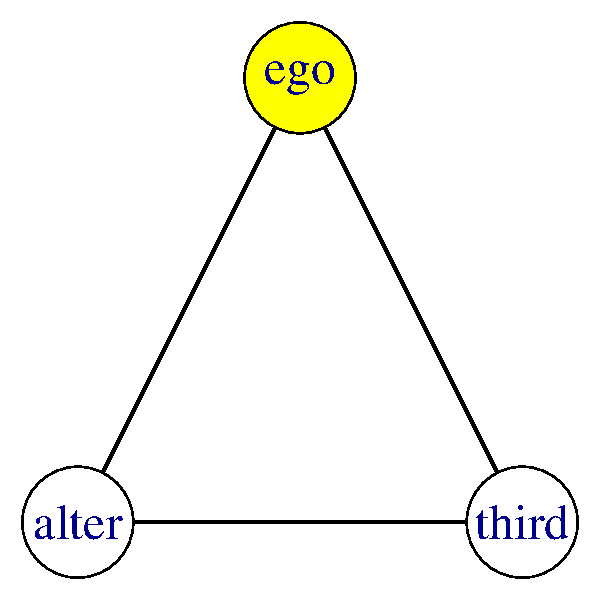
\includegraphics[width=2.5cm]{closedtriad}

\medskip

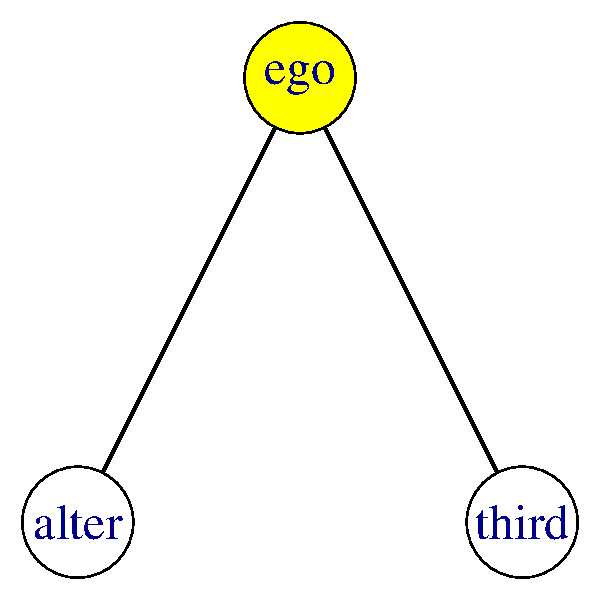
\includegraphics[width=2.5cm]{opentriad}

\end{columns}

\end{frame}

%------------------------------------------------

\begin{frame}
\frametitle{\insertsection}
\framesubtitle{\insertsubsection}

\begin{columns}
\column{.45\textwidth}

\begin{itemize}
\item At the level of an open triad, we can distinguish different types of {\color{blue}{brokerage roles}} \cite{Gould1989}
\item Roles are defined on the basis of {\color{blue}{groups}} to which the \textit{ego}, \textit{alter}, and \textit{third} belong
\end{itemize}

\column{.45\textwidth}
\centering
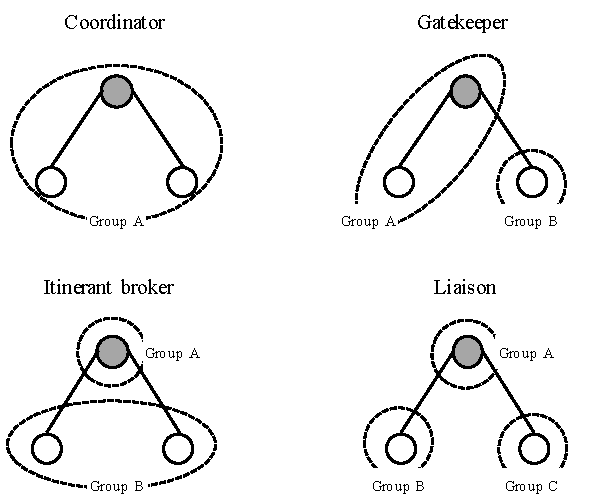
\includegraphics[width = \textwidth]{fernandez}
\end{columns}

\end{frame}

%------------------------------------------------

\begin{frame}
\frametitle{\insertsection}
\framesubtitle{\insertsubsection}

\begin{columns}
\column{.45\textwidth} 
\begin{itemize}
	\item The ego-network of a node includes all open and closed triads that contain the \textit{ego}
	\item For each triad we can assess the presence of {\color{blue}{structural holes}}
	\item To identify the {\color{blue}{number of triads}} we can count the number of possible ties, which is $(N-1)(N-2)/2$ in an undirected network
	\item Example: 6 triads and 5 structural holes
\end{itemize}

\column{.45\textwidth}
\centering
\includegraphics<1>[width=5cm]{base}
\includegraphics<2>[width=5cm]{egonet}
\end{columns}

\end{frame}

%------------------------------------------------



\begin{frame}
\frametitle{\insertsection}
\framesubtitle{Brokerage: Burt's measures of structural holes}

Ronald Burt introduced two main measures of {\color{blue}{structural holes}}. These are based on a node's ego-network \cite{Burt1992}

\medskip

\begin{itemize}
	\item Effective network size/efficiency
	\item Constraint
\end{itemize}
		
\end{frame}

%------------------------------------------------
\subsection{Effective network size/efficiency}
%------------------------------------------------

\begin{frame}
\frametitle{\insertsection}
\framesubtitle{\insertsubsection}


To define a node's {\color{blue}{effective network size}} and {\color{blue}{efficiency}}, we need to define the node's {\color{blue}{dyadic redundancy}}  with its primary contacts:

\begin{equation*}
dr_{ij} = \sum_{q}{p_{iq}m_{jq}} \;\;\;\;\;\; q \neq i, j
\end{equation*}

\begin{itemize}
	\item let's define $z_{ij}$ as the strength of the relation between node $i$ and node $j$ \\
	($z_{ij}=z_{ji}$ if the network is undirected)
	\item $p_{iq}$ is the proportional strength of node $i$'s relation with $q$: $\frac{z_{iq}+z_{qi}}{\sum_{j}(z_{ij}+z_{ji})}$
	\item $m_{jq}$ is the marginal strength of node $j$'s relation with $q$: $\frac{z_{jq}+z_{qj}}{max(z_{jk}+z_{kj})}$
	\item \textbf{Interpretation}
	\begin{itemize}
	\item $dr_{ij}$ provides indication of how many of the  actors in the ego-network of node $i$ are also tied to node $j$
	\item the higher is $dr_{ij}$, the more redundant is the tie of node $i$ with node $j$
	\end{itemize}
\end{itemize}
		
\end{frame}
%------------------------------------------------


\begin{frame}
\frametitle{\insertsection}
\framesubtitle{\insertsubsection}

\centering
\includegraphics<1>[width=5cm]{base}
\includegraphics<2>[width=5cm]{egonet}
\includegraphics<3>[width=5cm]{ps5}

\medskip

\onslide<2->\scalebox{0.8}{$p_{52} = \frac{z_{iq}+z_{qi}}{\sum_{j}(z_{ij}+z_{ji})} = \frac{(1+1)}{[(1+1)+(1+1)+(1+1)+(1+1)]}=0.25$}\\
\onslide<3->\scalebox{0.8}{$p_{53} = \frac{z_{iq}+z_{qi}}{\sum_{j}(z_{ij}+z_{ji})} = \frac{(1+1)}{[(1+1)+(1+1)+(1+1)+(1+1)]}=0.25$}\\
\onslide<3->\scalebox{0.8}{$p_{56} = \frac{z_{iq}+z_{qi}}{\sum_{j}(z_{ij}+z_{ji})} = \frac{(1+1)}{[(1+1)+(1+1)+(1+1)+(1+1)]}=0.25$}\\
\onslide<3->\scalebox{0.8}{$p_{57} = \frac{z_{iq}+z_{qi}}{\sum_{j}(z_{ij}+z_{ji})} = \frac{(1+1)}{[(1+1)+(1+1)+(1+1)+(1+1)]}=0.25$}
\end{frame}

%------------------------------------------------

\begin{frame}
\frametitle{\insertsection}
\framesubtitle{\insertsubsection}

\centering
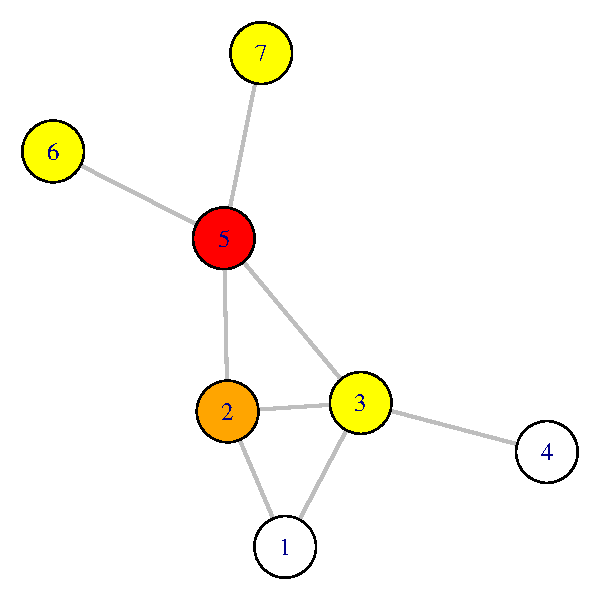
\includegraphics[width=5cm]{ms2}

\medskip

\scalebox{0.8}{$m_{23} = \frac{z_{jq}+z_{qj}}{max(z_{jk}+z_{kj})} =\frac{(1+1)}{max[(1+1), (1+1), (1+1)]}=1$}\\
\scalebox{0.8}{$m_{26} = \frac{z_{jq}+z_{qj}}{max(z_{jk}+z_{kj})} = \frac{0}{max[(1+1), (1+1), (1+1)]}=0$}\\
\scalebox{0.8}{$m_{27} = \frac{z_{jq}+z_{qj}}{max(z_{jk}+z_{kj})} = \frac{0}{max[(1+1), (1+1), (1+1)]}=0$}

\end{frame}

%------------------------------------------------


\begin{frame}
\frametitle{\insertsection}
\framesubtitle{\insertsubsection}

\centering
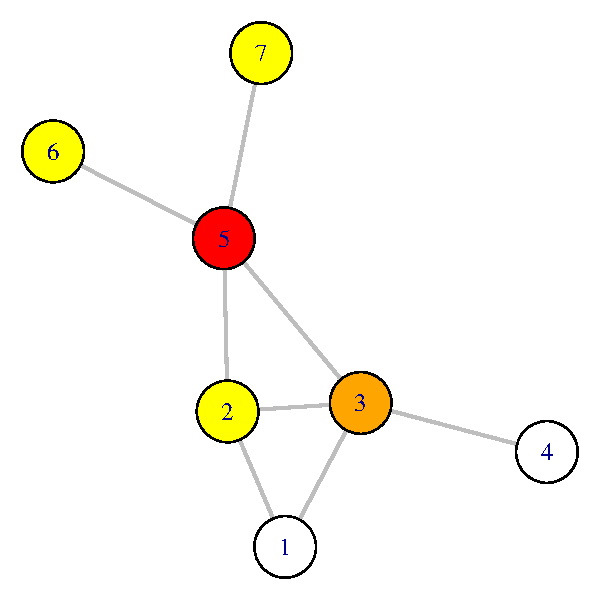
\includegraphics[width=5cm]{ms3}

\medskip

\scalebox{0.8}{$m_{32} = \frac{z_{jq}+z_{qj}}{max(z_{jk}+z_{kj})} =\frac{(1+1)}{max[(1+1), (1+1), (1+1), (1+1)]}=1$}\\
\scalebox{0.8}{$m_{36} = \frac{z_{jq}+z_{qj}}{max(z_{jk}+z_{kj})} = \frac{0}{max[(1+1), (1+1), (1+1), (1+1)]}=0$}\\
\scalebox{0.8}{$m_{37} = \frac{z_{jq}+z_{qj}}{max(z_{jk}+z_{kj})} = \frac{0}{max[(1+1), (1+1), (1+1), (1+1)]}=0$}\\

\end{frame}

%------------------------------------------------

\begin{frame}
\frametitle{\insertsection}
\framesubtitle{\insertsubsection}

\centering
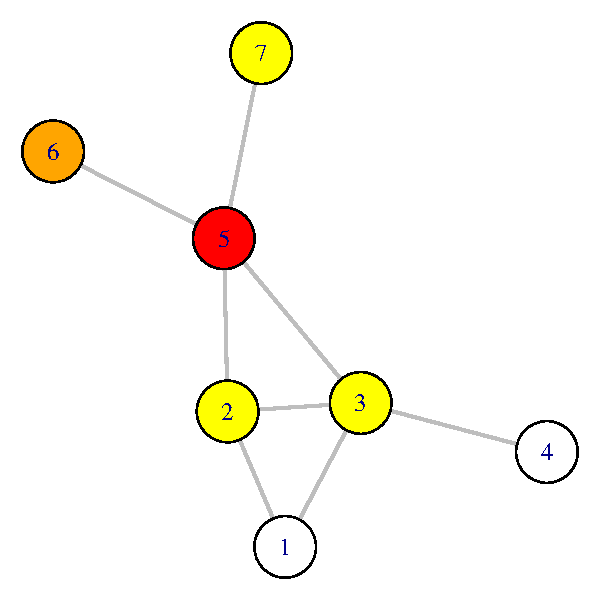
\includegraphics[width=5cm]{ms6}

\medskip

\scalebox{0.8}{$m_{62} = \frac{z_{jq}+z_{qj}}{max(z_{jk}+z_{kj})} = \frac{0}{max[(1+1)]}=0$}

\scalebox{0.8}{$m_{63} = \frac{z_{jq}+z_{qj}}{max(z_{jk}+z_{kj})} = \frac{0}{max[(1+1)]}=0$}

\scalebox{0.8}{$m_{67} = \frac{z_{jq}+z_{qj}}{max(z_{jk}+z_{kj})} = \frac{0}{max[(1+1)]}=0$}


\end{frame}

%------------------------------------------------

\begin{frame}
\frametitle{\insertsection}
\framesubtitle{\insertsubsection}

\centering
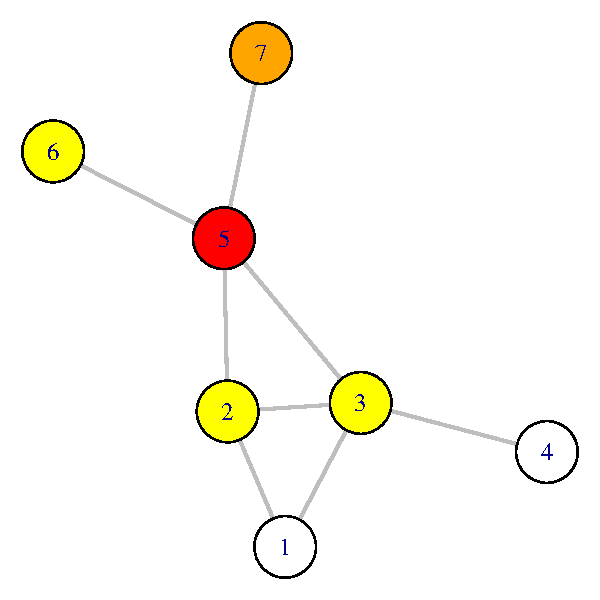
\includegraphics[width=5cm]{ms7}

\medskip


\scalebox{0.8}{$m_{72} = \frac{z_{jq}+z_{qj}}{max(z_{jk}+z_{kj})} = \frac{0}{max[(1+1)]}=0$}

\scalebox{0.8}{$m_{73} = \frac{z_{jq}+z_{qj}}{max(z_{jk}+z_{kj})} = \frac{0}{max[(1+1)]}=0$}

\scalebox{0.8}{$m_{76} = \frac{z_{jq}+z_{qj}}{max(z_{jk}+z_{kj})} = \frac{0}{max[(1+1)]}=0$}


\end{frame}

%------------------------------------------------

\begin{frame}
\frametitle{\insertsection}
\framesubtitle{\insertsubsection}

\centering
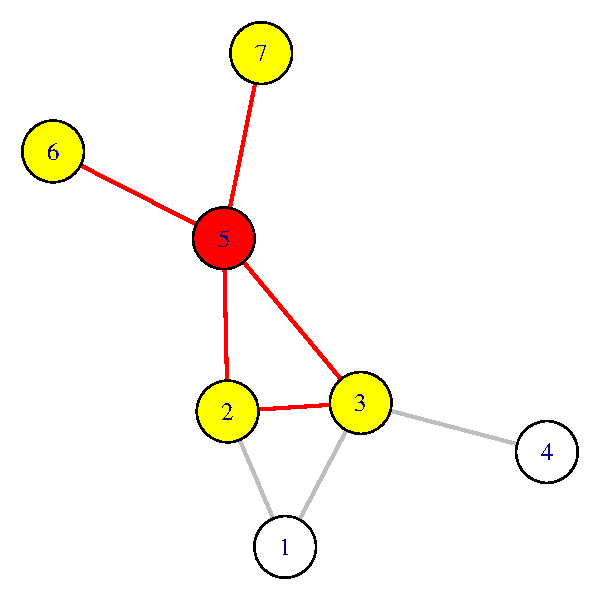
\includegraphics[width=5cm]{egonet}

\medskip

\scalebox{0.8}{$dr_{52} = \sum_{q}{p_{iq}m_{jq}} = p_{53}m_{23}+p_{56}m_{26}+p_{57}m_{27} = 0.25*1+0.25*0+ 0.25*0 = 0.25$}\\
\scalebox{0.8}{$dr_{53} = \sum_{q}{p_{iq}m_{jq}} = p_{52}m_{32}+p_{56}m_{36}+p_{57}m_{37} = 0.25*1+0.25*0+0.25*0 = 0.25$}\\
\scalebox{0.8}{$dr_{56} = \sum_{q}{p_{iq}m_{jq}} = p_{52}m_{62}+p_{53}m_{63}+p_{57}m_{67} = 0.25*0+0.25*0+0.25*0 = 0$}\\
\scalebox{0.8}{$dr_{57} = \sum_{q}{p_{iq}m_{jq}} = p_{52}m_{72}+p_{53}m_{73}+p_{56}m_{76} = 0.25*0+0.25*0+0.25*0 = 0$}

\end{frame}

%------------------------------------------------

\begin{frame}
\frametitle{\insertsection}
\framesubtitle{\insertsubsection}


A node's {\color{blue}{effective network size}} is the sum of one minus all the dyadic redundancy values of the node with the other nodes in its ego-network \cite{Burt1992}

\begin{equation*}
EN_{i} = \sum_{j}{[1 - \sum_{q}{p_{iq}m_{qj}}]} = \sum_{j}{[1 - dr_{ij}]} \;\;\;\;\;\; q \neq i, j
\end{equation*}

\begin{itemize}
	\item $EN_{i}$ ranges from $0$ to $N-1$
	\item $EN_{i}/N$ is defined {\color{blue}{efficiency}} ($EFF_{i}$)
\end{itemize}

\end{frame}

%------------------------------------------------

\begin{frame}
\frametitle{\insertsection}
\framesubtitle{\insertsubsection}

\centering
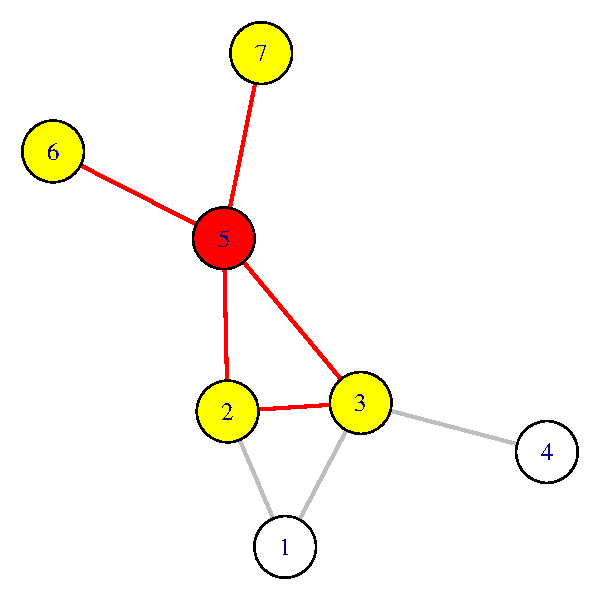
\includegraphics[width=5cm]{egonet}

\medskip

\scalebox{0.8}{$EN_{5} = [1 - dr_{52}] + [1 - dr_{53}] + [1 - dr_{56}]  + [1 - dr_{57}] = [1 - 0.25] + [1 - 0.25] + [1 - 0] + [1 - 0]= 3.5$}

\end{frame}

%------------------------------------------------

\begin{frame}
\frametitle{\insertsection}
\framesubtitle{\insertsubsection}

\begin{columns}
	\column{.45\textwidth}
	\centering 
	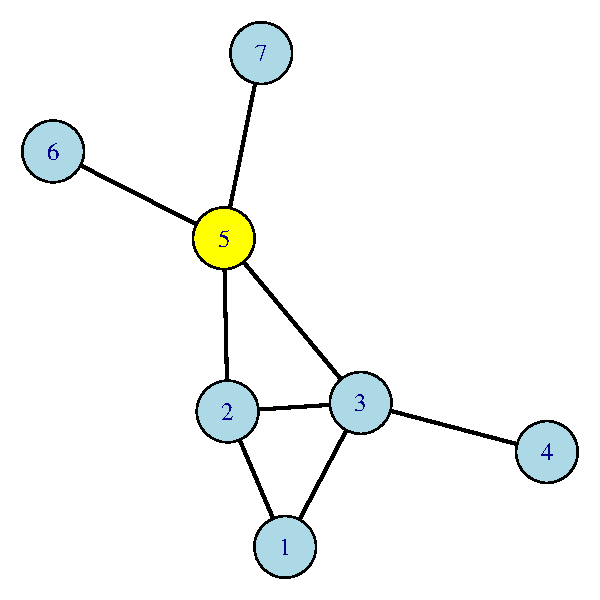
\includegraphics[width=5cm]{effective}
	
	\column{.45\textwidth}
	
	\small
	\renewcommand{\arraystretch}{1.5}
	\begin{table}
	\begin{tabular}{ccc}
		\toprule
	$n_i$ & $EN(n_i)$ & $EFF(n_i)$\\
	\hline
	1 & 1.00 & 0.14\\
	2 & 1.67 & 0.24\\
	3 & 3.00 & 0.43\\
	4 & 1.00 & 0.14\\
	5 & 3.50 & 0.50\\
	6 & 1.00 & 0.14\\
	7 & 1.00 & 0.14\\
	\bottomrule
	\end{tabular}
	\end{table}
\end{columns}
\end{frame}
%------------------------------------------------

\begin{frame}
\frametitle{\insertsection}
\framesubtitle{\insertsubsection}


\centering 
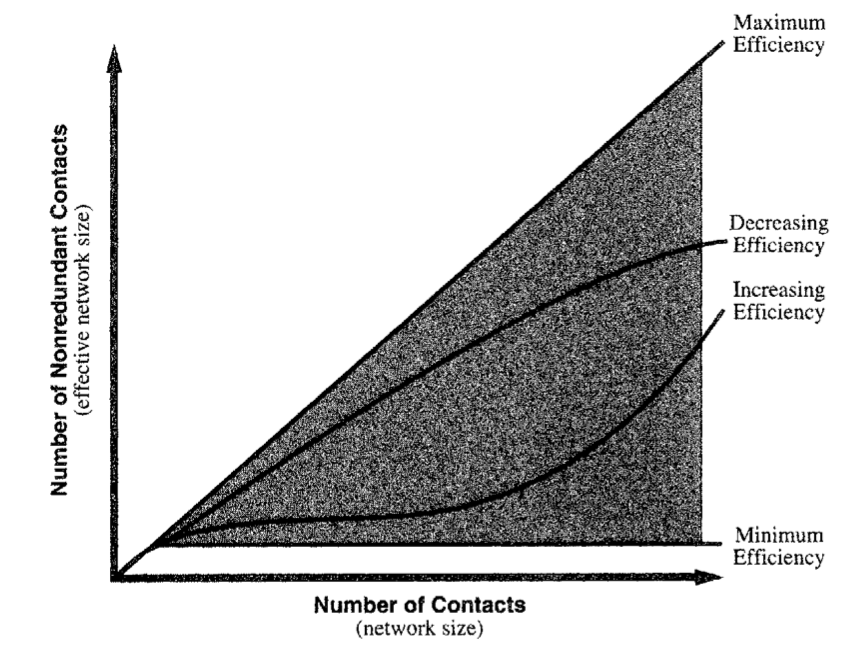
\includegraphics[width = 0.7\textwidth]{efficiency_burt}\\
\tiny{Source: \cite{Burt1992}}

\end{frame}

%------------------------------------------------
\subsection{Constraint}
%------------------------------------------------

\begin{frame}
\frametitle{\insertsection}
\framesubtitle{\insertsubsection}

To define a node's {\color{blue}{constraint}} we need to define the node's {\color{blue}{dyadic constraint}} with its primary contacts:

\begin{equation*}
dc_{ij} = \left(p_{ij} + \sum_{q}{p_{iq}p_{jq}}\right)^2 \;\;\;\;\;\; q \neq i, j
\end{equation*}

\begin{itemize}
	\item let's define $z_{ij}$ as the strength of the relation between node $i$ and node $j$ \\
	($z_{ij}=z_{ji}$ if the network is undirected)
	\item $p_{iq}$ is the proportional strength of node $i$'s relation with $q$: $\frac{z_{iq}+z_{qi}}{\sum_{j}(z_{ij}+z_{ji})}$
	\item $p_{jq}$ is the proportional strength of node $j$'s relation with $q$: $\frac{z_{jq}+z_{qj}}{\sum_{k}(z_{jk}+z_{kj})}$
	\item $dc_{ij}$ provides indication on the extent to which $j$ is more or less connected to nodes to which $i$ is strongly connected
	\item \textbf{Interpretation}
	\begin{itemize}
	\item $dc_{ij}$ provides indication of the extent to which the tie between node $i$ and node $j$ ``constraints'' node $i$
	\item the higher is $dc_{ij}$, the more constrained is node $i$ by node $j$
		\item $dc_{ij} = 1$ when node $j$ is the only connection of $i$
	\end{itemize}
\end{itemize}
		
\end{frame}

%------------------------------------------------

\begin{frame}
\frametitle{\insertsection}
\framesubtitle{\insertsubsection}
\centering
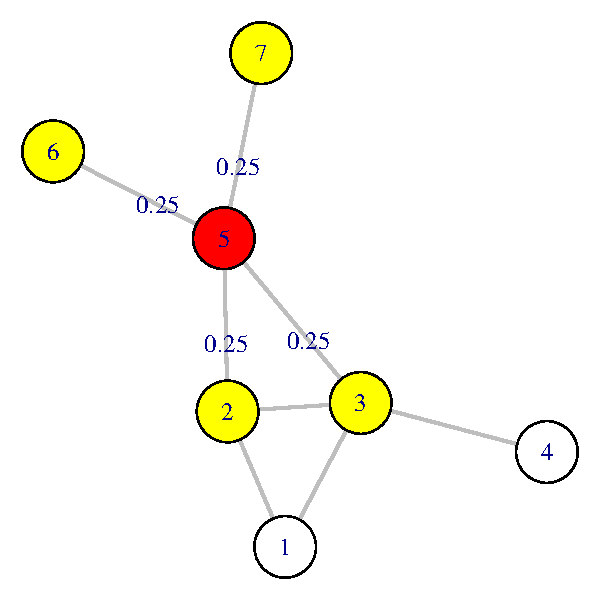
\includegraphics[width=5cm]{ps5}

\scalebox{0.8}{$p_{5q} = \frac{z_{iq}+z_{qi}}{\sum_{j}(z_{ij}+z_{ji})} = \frac{(1+1)}{[(1+1)+(1+1)+(1+1)+(1+1)]}=0.25 \;\;\;\;\;\; q={2,3,6,7}$}
	
\end{frame}

%------------------------------------------------

\begin{frame}
\frametitle{\insertsection}
\framesubtitle{\insertsubsection}
\centering
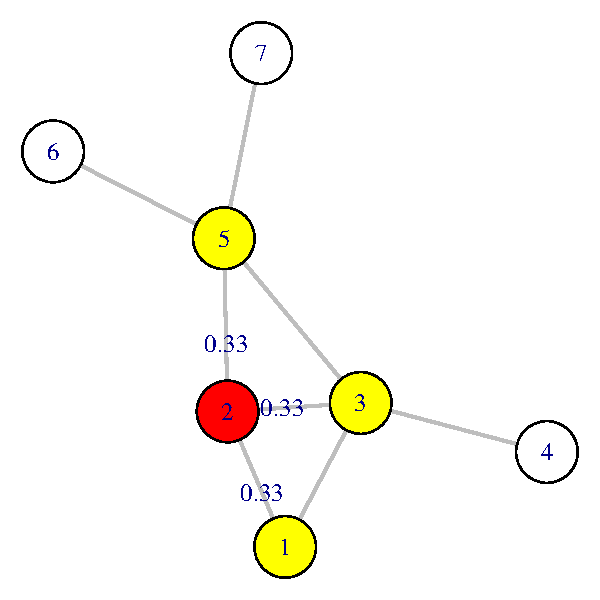
\includegraphics[width = 0.25\textwidth]{ps2}
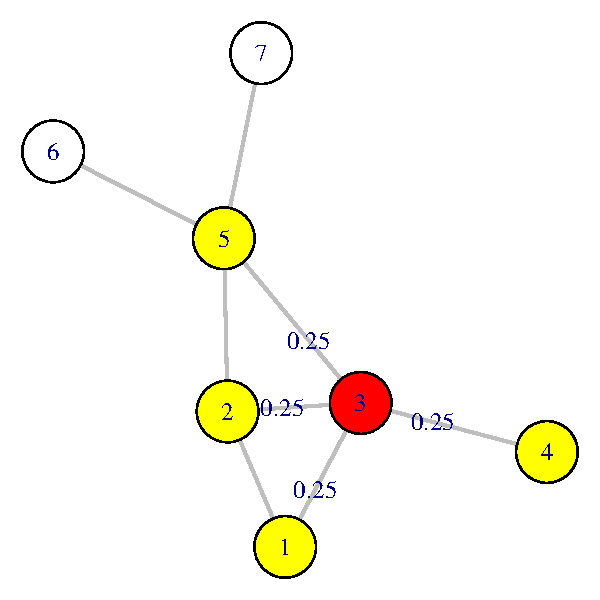
\includegraphics[width = 0.25\textwidth]{ps3}
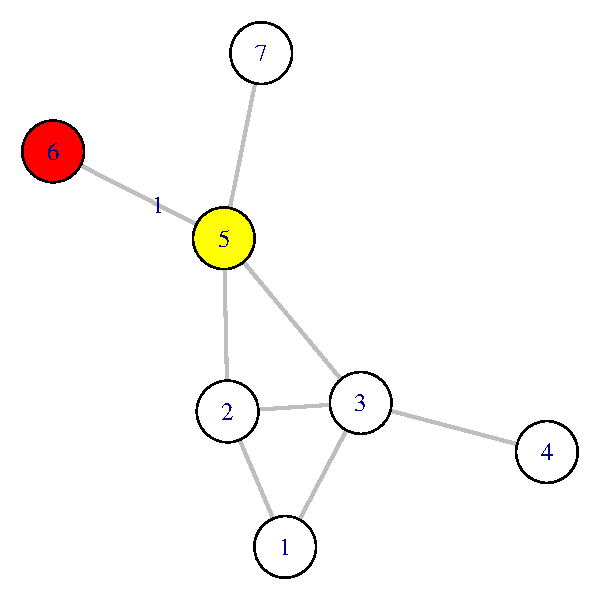
\includegraphics[width = 0.25\textwidth]{ps6}
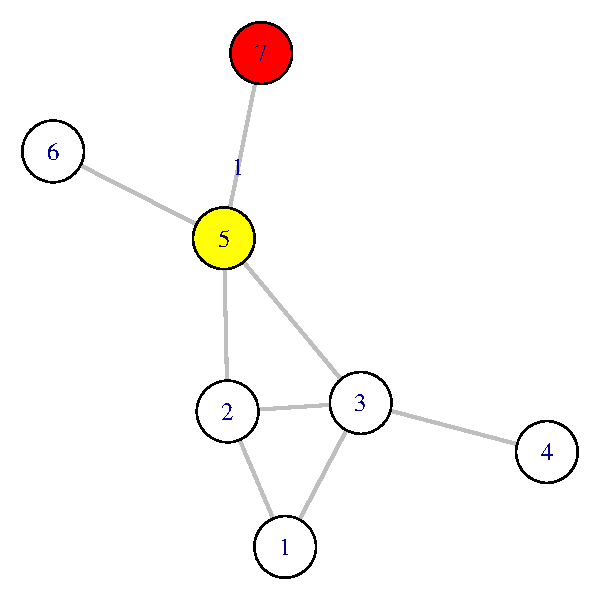
\includegraphics[width = 0.25\textwidth]{ps7}

\medskip

\scalebox{0.8}{$p_{2q} = \frac{z_{iq}+z_{qi}}{\sum_{j}(z_{ij}+z_{ji})} = \frac{(1+1)}{[(1+1)+(1+1)+(1+1)]}=0.33 \;\;\;\;\;\; q={1,3,5}$}

\scalebox{0.8}{$p_{3q} = \frac{z_{iq}+z_{qi}}{\sum_{j}(z_{ij}+z_{ji})} = \frac{(1+1)}{[(1+1)+(1+1)+(1+1)+(1+1)]}=0.25 \;\;\;\;\;\; q={1,2,4,5}$}

\scalebox{0.8}{$p_{6q} = \frac{z_{iq}+z_{qi}}{\sum_{j}(z_{ij}+z_{ji})} = \frac{(1+1)}{[(1+1)]}=1.00 \;\;\;\;\;\; q={5}$}

\scalebox{0.8}{$p_{7q} = \frac{z_{iq}+z_{qi}}{\sum_{j}(z_{ij}+z_{ji})} = \frac{(1+1)}{[(1+1)]}=1.00 \;\;\;\;\;\; q={5}$}

\end{frame}

%------------------------------------------------

\begin{frame}
\frametitle{\insertsection}
\framesubtitle{\insertsubsection}
\centering
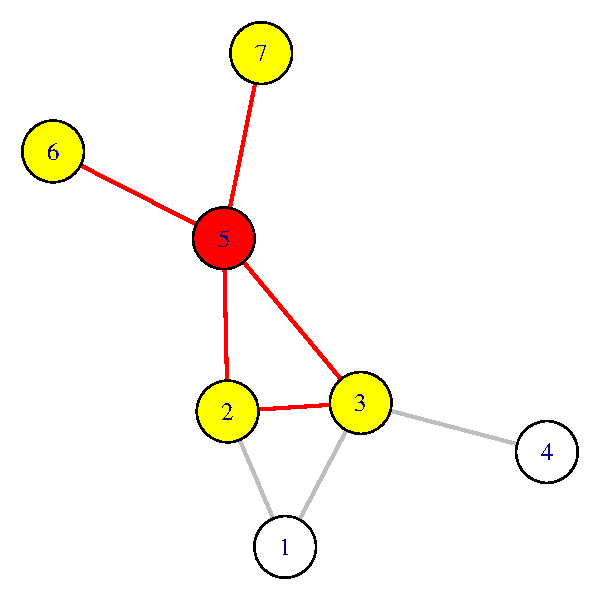
\includegraphics[width=5cm]{egonet}

\medskip

\scalebox{0.8}{$dc_{52} = \left(p_{52}+p_{53}p_{23}+p_{56}p_{26}+p_{57}p_{27}\right)^2 = \left(0.25 + 0.25 * 0.33 +  0.25 * 0 +  0.25 * 0\right)^2 = 0.1111$}\\
\scalebox{0.8}{$dc_{53} = \left(p_{53}+p_{52}p_{32}+p_{56}p_{36}+p_{57}p_{37}\right)^2 = \left(0.25 + 0.25 * 0.25 +  0.25 * 0 +  0.25 * 0\right)^2 = 0.0976$}\\
\scalebox{0.8}{$dc_{56} = \left(p_{56}+p_{52}p_{62}+p_{53}p_{63}+p_{57}p_{67}\right)^2 = \left(0.25 + 0.25 * 0 +  0.25 * 0 +  0.25 * 0\right)^2 = 0.0625$}\\
\scalebox{0.8}{$dc_{57} = \left(p_{57}+p_{52}p_{72}+p_{53}p_{73}+p_{56}p_{76}\right)^2 = \left(0.25 + 0.25 * 0 +  0.25 * 0 +  0.25 * 0\right)^2 = 0.0625$}	

\end{frame}

%------------------------------------------------


\begin{frame}
\frametitle{\insertsection}
\framesubtitle{\insertsubsection}

A node's {\color{blue}{constraint}} is the sum of all dyadic constraint values of the node with the other nodes in the ego-network \cite{Burt1992}

\begin{equation*}
C_{i} = \sum_{j}{dc_{ij}} 
\end{equation*}

\begin{itemize}
	\item $C_{i}$ depend on the size and density of the ego network (it tends to be higher in small and dense networks)
	\item The density of the ego-network is also used to assess a node's constrain
\end{itemize}
		
\end{frame}

%------------------------------------------------

\begin{frame}
\frametitle{\insertsection}
\framesubtitle{\insertsubsection}

\centering
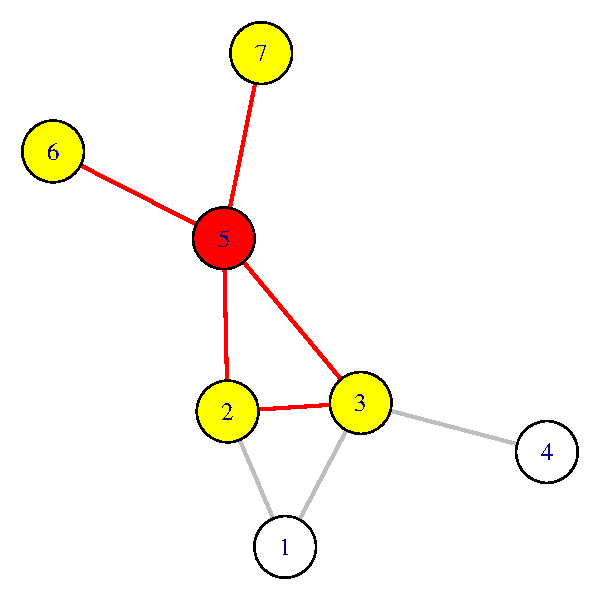
\includegraphics[width=5cm]{egonet}

\medskip

\scalebox{0.8}{$C_{5} =  \sum_{j}{dc_{ij}} = dc_{52} + dc_{53} + dc_{56} + dc_{57} = 0.1111+0.0976+0.0625+0.0625 = 0.3337$}

\end{frame}

%------------------------------------------------

\begin{frame}
\frametitle{\insertsection}
\framesubtitle{\insertsubsection}

\begin{columns}
	\column{.45\textwidth} 
         \centering 
	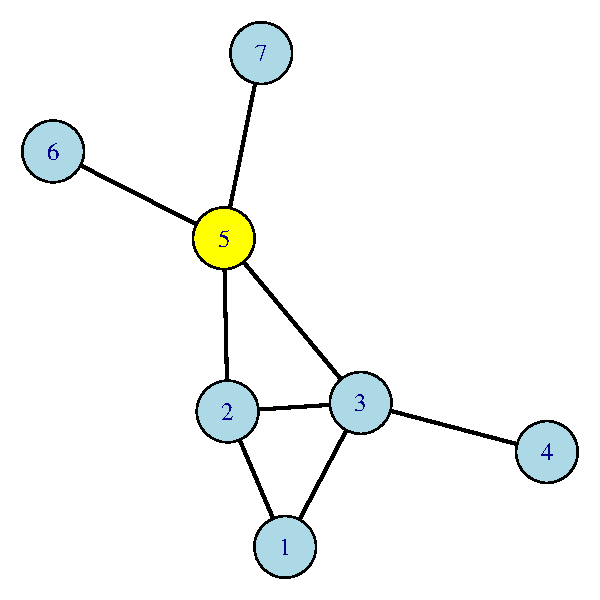
\includegraphics[width=5cm]{constraint}
	
	\column{.45\textwidth}
	\small
	\renewcommand{\arraystretch}{1.5}
	\begin{table}
	\begin{tabular}{cc}
		\toprule
	$n_i$ & $C(n_i)$\\
	\hline
	1 & 0.83\\
	2 & 0.69\\
	3 & 0.48\\
	4 & 1.00\\
	5 & 0.33\\
	6 & 1.00\\
	7 & 1.00\\
	\bottomrule
	\end{tabular}
	\end{table}
\end{columns}
\end{frame}

%------------------------------------------------

\begin{frame}[fragile]
\frametitle{\insertsection}
\framesubtitle{\insertsubsection \vspace{0.1cm} (example)}

\begin{columns}[c]

\column{.3\textwidth}
\begin{minipage}[c][.5\textheight][c]{\linewidth}


Country alliances
\begin{itemize}
\item 1816-2012 period     
\item 3,222 alliances
\item Nodes' size proportional to nodes' constraint
\end{itemize}

\medskip
\medskip

\end{minipage}	   


\column{.7\textwidth}
\begin{minipage}[c][.5\textheight][c]{\linewidth}
\centering

\only<1>{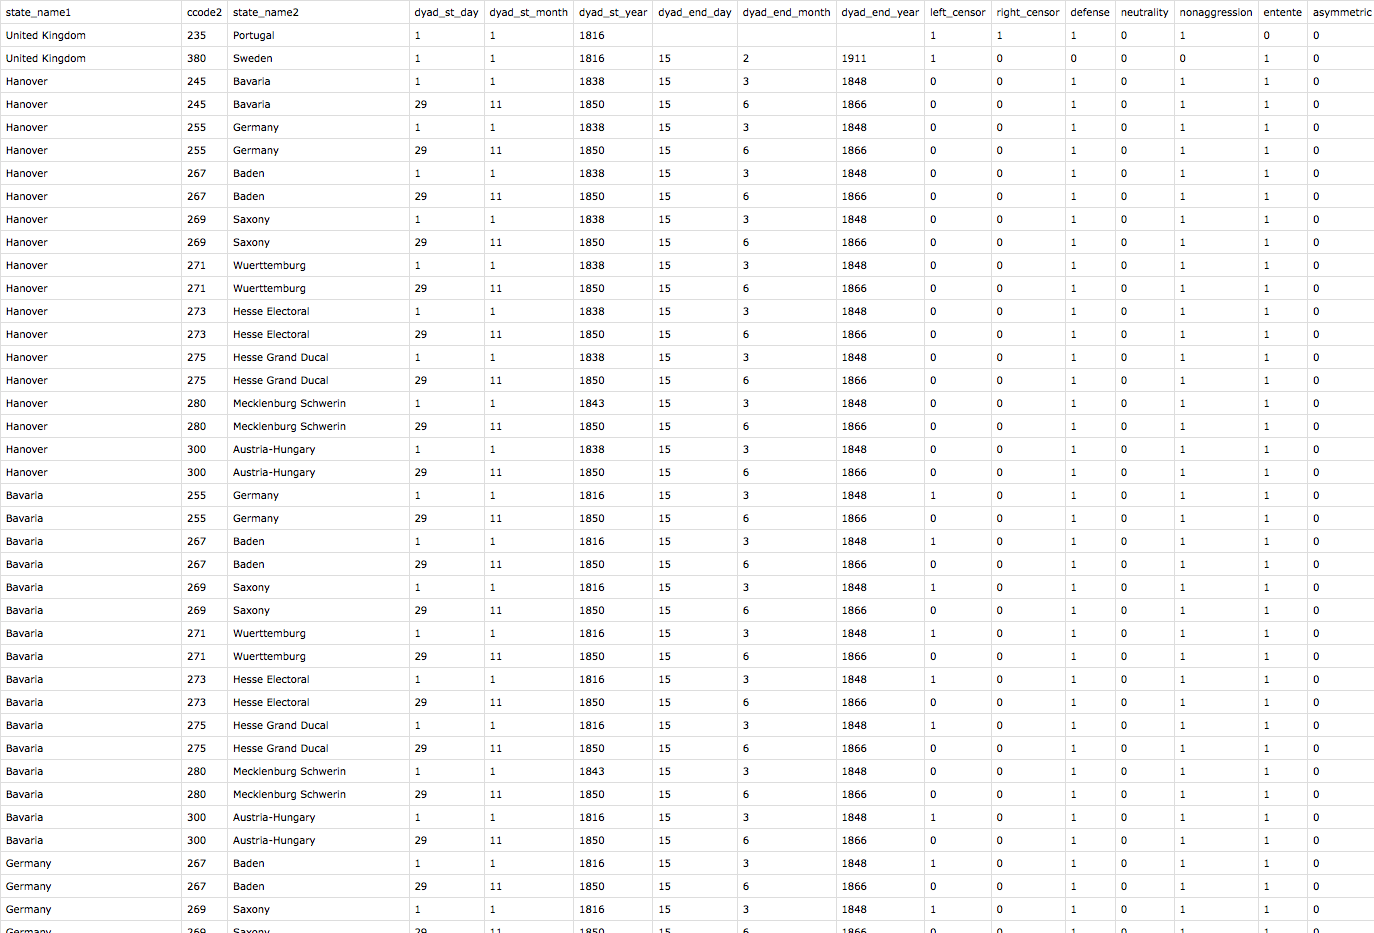
\includegraphics[width = 0.9\textwidth, frame]{alliances_data}\\
\tiny{Source: \url{http://www.correlatesofwar.org/}}}

\only<2>{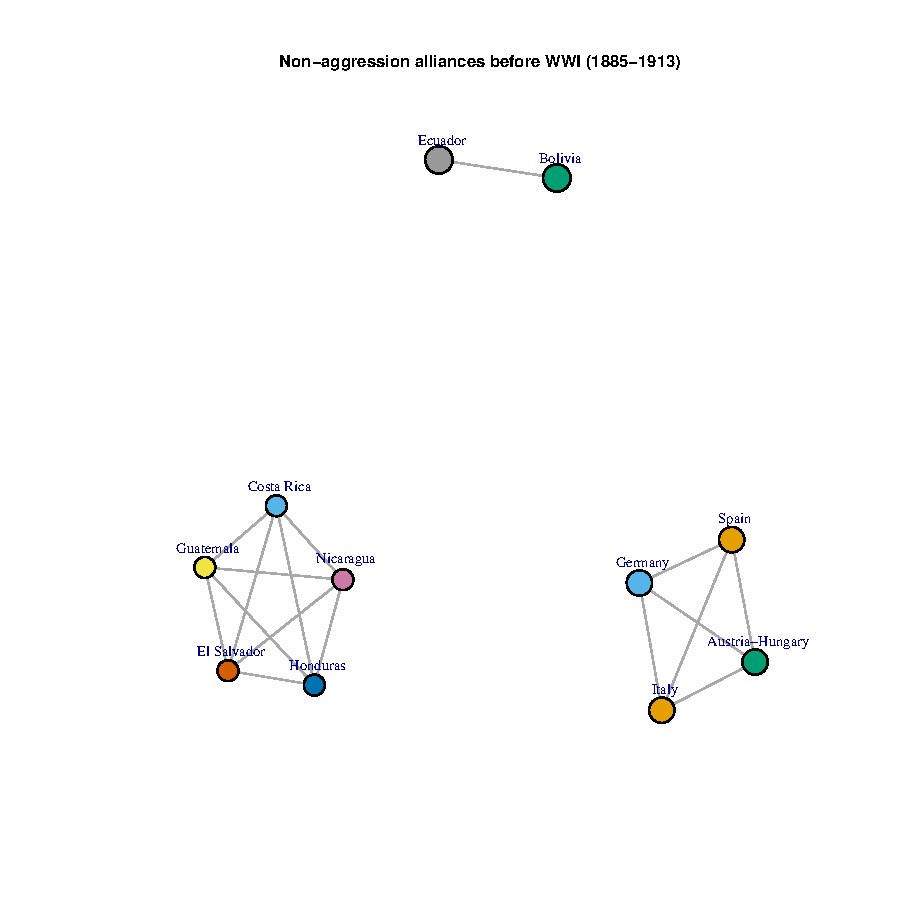
\includegraphics[width = 1.1\textwidth]{alliances_before_wwi.pdf}}

\only<3>{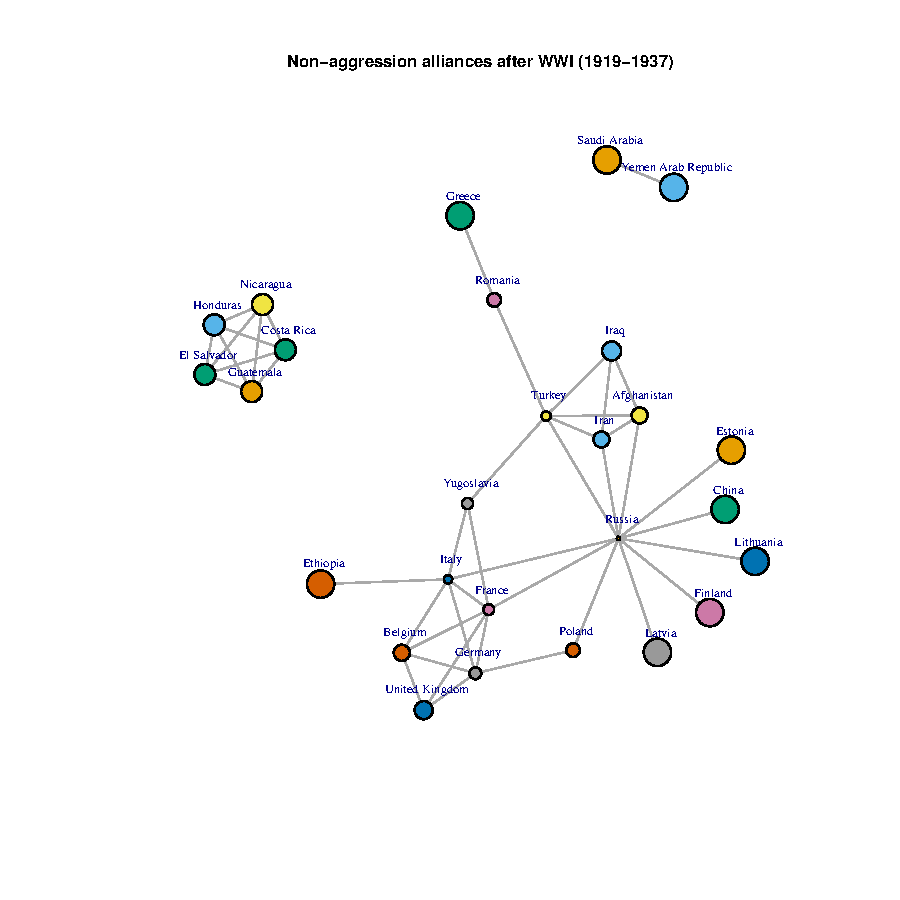
\includegraphics[width = 1.1\textwidth]{alliances_after_wwi.pdf}}

\end{minipage}

\end{columns}

\end{frame}
  

%------------------------------------------------
\begin{frame}[fragile]
\frametitle{\insertsection}
\framesubtitle{\insertsubsection \vspace{0.1cm} (example)}

\lstinputlisting[language = R, firstline = 15, lastline = 49]{handouts_script/L6_script_handouts.R}

\end{frame}
  

%------------------------------------------------

\begin{frame}
\frametitle{\insertsection}
\framesubtitle{Network density}


\centering 
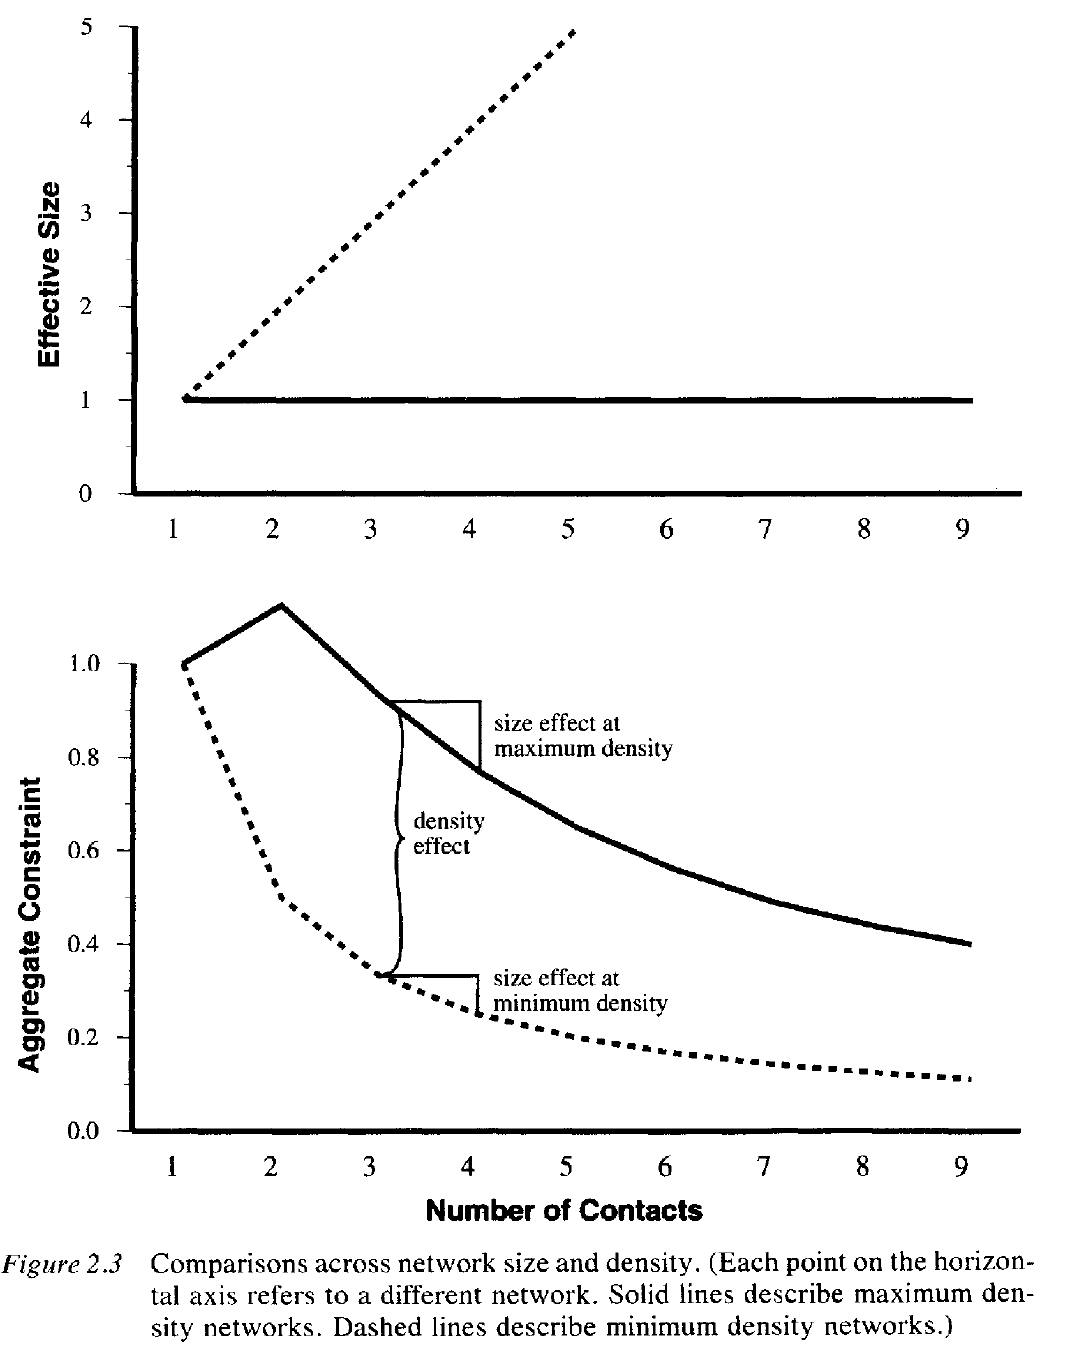
\includegraphics[width = 0.5\textwidth]{burt_density}\\
\tiny{Source: \cite{Burt1992}}

\end{frame}


%------------------------------------------------

\begin{frame}
\frametitle{\insertsection}
\framesubtitle{Summary}

\small
\begin{table}
\begin{tabular}{p{3cm}p{7.5cm}}
\toprule
\textbf{Measure}        & \textbf{Interpretation} \\
\hline
\\
Brokerage roles         & Coordinator, gatekeeper, itinerant broker, liaison\\
\\
Effective network size  & To what extent a node share ties with other nodes?\\
\\
Constraint              & To what extent a node's action is constrained by other nodes in the ego-network?\\
\\
\bottomrule
\end{tabular}
\end{table}
\end{frame}

%------------------------------------------------




%=======================================================
%	Questions
%=======================================================
\bgroup
\setbeamercolor{background canvas}{bg = orange}
\begin{frame}[plain]{}
\begin{center}
\color{white}{\Huge Questions}
\end{center}
\end{frame}
\egroup







%%=======================================================
%	Next time ...
%%=======================================================
\section*{Next time ...}

%------------------------------------------------

\bgroup
\setbeamercolor{background canvas}{bg = navyblue}
\begin{frame}[plain]{}
\begin{center}
\color{white}{\Huge\insertsection}
\end{center}
\end{frame}
\egroup

%------------------------------------------------

\begin{frame}
\frametitle{\insertsection}

\begin{itemize}

\item 	\textbf{Seminar: Descriptive network analysis C}
	\begin{itemize}
	\item Assessment of node-level measures (brokerage measures)
	\end{itemize}
	

\medskip
\medskip

\item 	\textbf{Lecture: Principles of infographics}
	\begin{itemize}
	\item Principles and good practices to generate infographics
	\item Network layout algorithms
	\end{itemize}

		
\end{itemize}

\end{frame}

%------------------------------------------------








%=======================================================
%	References
%=======================================================
\begin{frame}[allowframebreaks]
\frametitle{References}
\tiny
\bibliographystyle{apalike}
\bibliography{references(2).bib}
\end{frame}
%------------------------------------------------




\end{document}